
All test have been run on the same machine with the following specifications: 


\begin{itemize}
    \item \textbf{CPU} - Intel Core i7-4770k 4-Core (8 threads) 3.50 GHz
    \item \textbf{RAM} - Corsair 16 GB DDR3 1600 MHz 
    \item \textbf{OS} - Windows 10 Pro 64-bit
    \item \textbf{JVM} - Oracle Corporation 16.0
\end{itemize}
\vspace{0.5cm}
\subsection{Original Program Introduction}



\label{sec:2.1}
The Original Program to be optimized supplied by the school (the link in the assignment description) have the following description:
\begin{displayquote}
\emph{Simple program used to illustrate performance problems. You should be able to optimize this program to run about twice as fast. \cite{cph}.} 
\end{displayquote}

The program source consists of the foundation trilogy by Isaac Asimov (roughly 25.000 lines of text) and a single Java file.
The file reads the text and returns the frequencies of the letters within the text.

The Java program is purposefully written in an inefficient way. It has two helper methods and at its core it presents a list of the letter frequencies between a-zA-Z. 

Below you can find a sample of the output of the program:

\begin{table}[h]
    \centering
    \begin{tabular}{cc}
    Letter & Frequencies \\
    E      & 118313      \\
    T      & 87190       \\
    A      & 76011       \\
    O      & 74907       \\
    N      & 67908       \\
    ...    & ...         \\
    K      & 6630        \\
    X      & 1457        \\
    Q      & 1017        \\
    J      & 806         \\
    Z      & 674        
    \end{tabular}
    \caption{The 5 most and least frequent letters in the dataset}
\end{table}

\vspace{0.5cm}
\subsection{Current Performance}
\label{sec:2.2}
We measured the program using the Mark5 method supplied by Sestoft.\cite{sestoft} \newline
This is the current console readings when the program is run without any changes to the code. 
So a baseline run time of 51 miliseconds with a standard deviation of 1.07 miliseconds. 
\lstset{
tabsize = 4, 
showstringspaces = false, 
numbers = none, 
rulecolor = \color{white}, 
basicstyle = \small \ttfamily, 
breaklines = true, 
numberstyle = \small,
}
\begin{lstlisting}[language = Java , firstnumber = last , escapeinside={(*@}{@*)}]
    -------------------------------------------
    Mean              Sdev               Count
    -------------------------------------------
    60,2 ms +/-    20,39 ms          2
    54,7 ms +/-     4,41 ms          4
    51,4 ms +/-     1,62 ms          8
    51,1 ms +/-     1,90 ms         16
    50,7 ms +/-     0,28 ms         32
    50,7 ms +/-     0,64 ms         64
    51,0 ms +/-     1,07 ms        128
    -------------------------------------------
\end{lstlisting}

\newpage
\subsection{Bottleneck(s)}
\label{sec:2.3}
Profiling with the Java Flight Recorder in IntelliJ gives us the following indication of the programs shortcommings:
\begin{figure}[H]
    \centering\
    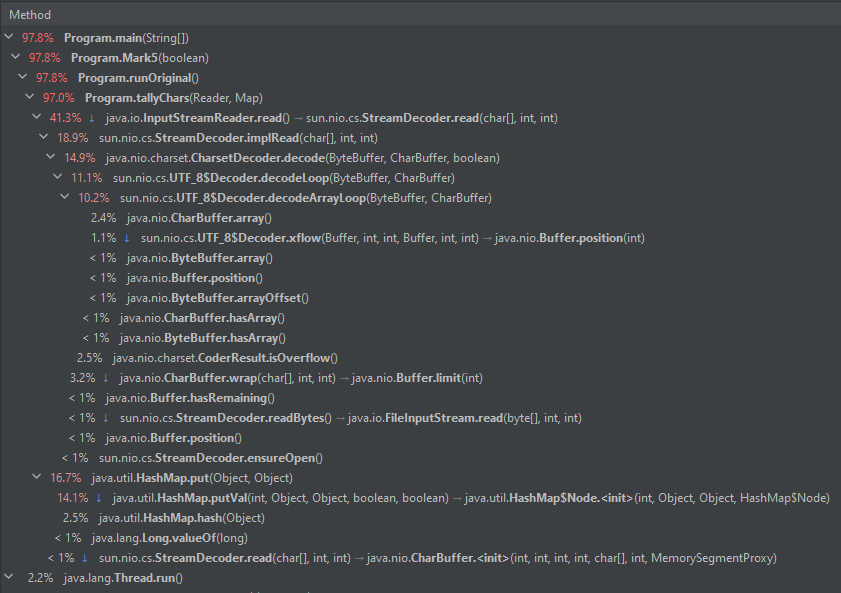
\includegraphics[width = 0.8\textwidth ]{figures/profile1.PNG}
    \caption{Java Fligt Recorder Profile 1}
    \label{fig:p1}
\end{figure}
As it can be seen, most of the ressources are spent within the \emph{tallyChars()} method. We decided to start looking at the two following areas of the program:
\begin{itemize}
    \item The file reading
    \item The HashMap 
\end{itemize}

\vspace{0.5cm}
\subsection{Hypothesis}
\label{sec:2.4}
We suspected that the file reading was slowed down a lot by only using the \emph{FileReader}, since the \emph{FileReader} reads a few bytes at a time and a \emph{BufferedReader} wrapped around a \emph{FileReader} will buffer a whole line and keep it ready. 
The use of \emph{HashMap} seemed to us to be doing a lot of unnecessary work and we thought that an optimization of that could improve the overall run time some amount.  

\vspace{0.5cm}
\subsection{Solution(s)}
\label{sec:2.5}

We have done the following, all of which can be seen in the code (except the \emph{BufferedReader} which have been further optimized):
\begin{itemize}
    \item Implementing the wrapper \emph{BufferedReader}
    \item Optimization of the \emph{HashMap} and using \emph{ArrayList}
    \item Further optimization of the file reading with the use of \emph{java.nio.file.Files}
\end{itemize}


\subsection{Optimized Performance}
\label{sec:2.6}
In this section the documentation for each improvement can be seen, along with our thoughts about the changes. 
\subsubsection{BufferedReader}
\label{sec:2.6.1}
The use of a BufferedReader alone have increased the program mean runtime by \textbf{40,87\%}. Looking at the Profile produced by the Java Flight Recorder in IntelliJ after this change, confirms that this was an actual issue with the original code.
\begin{lstlisting}[language = Java , firstnumber = last , escapeinside={(*@}{@*)}]
    -------------------------------------------
    Mean              Sdev               Count
    -------------------------------------------
    26688810,0 ns +/- 8156130,62          2
    21170010,0 ns +/- 1636441,34          4
    20378076,3 ns +/- 165036,89           8
    20086596,9 ns +/- 70131,53            16
    20113604,4 ns +/- 95585,47            32
    20121626,1 ns +/- 132419,65           64
    20107895,8 ns +/- 106333,91           128
    20220584,5 ns +/- 145384,37           256
    20213537,6 ns +/- 40180,77            512
    -------------------------------------------
\end{lstlisting}

\begin{figure}[H]
    \centering\
    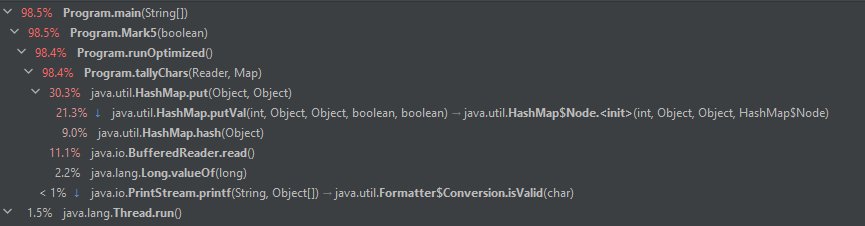
\includegraphics[width = 0.8\textwidth ]{figures/profile2.PNG}
    \caption{Java Fligt Recorder Profile 2}
    \label{fig:p2}
\end{figure}

\subsubsection{HashMap refactoring}
\label{sec:2.6.2}
After modifying \emph{HashMap} and the methods \emph{tallyChars()} and \emph{print\_tally()} we are now at an \textbf{42,37\%} overall optimization.
\begin{lstlisting}[language = Java , firstnumber = last , escapeinside={(*@}{@*)}]
    -------------------------------------------
    Mean              Sdev               Count
    -------------------------------------------
    24734475,0 ns +/- 6057492,36          2
    20550197,5 ns +/- 1135309,37          4
    19897790,0 ns +/- 169372,90           8
    19688542,5 ns +/- 71463,82            16
    20048747,5 ns +/- 322151,07           32
    19751591,6 ns +/- 133747,31           64
    19704611,6 ns +/- 73574,46            128
    19760670,4 ns +/- 108017,90           256
    19701593,6 ns +/- 47694,74            512
    -------------------------------------------
\end{lstlisting}

\begin{figure}[H]
    \centering\
    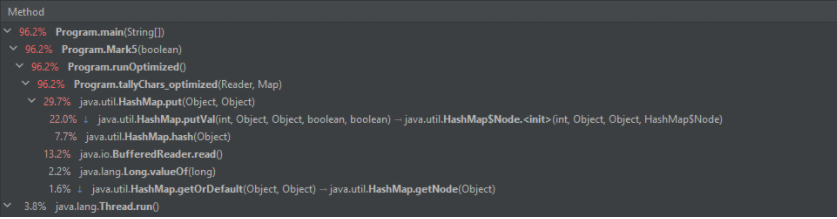
\includegraphics[width = 0.8\textwidth ]{figures/profile3.PNG}
    \caption{Java Fligt Recorder Profile 3}
    \label{fig:p3}
\end{figure}

\subsubsection{java.nio.file.Files}
\label{sec:2.6.3}

After changing from \emph{BufferedReader} to this lambda expression from \emph{java.nio.file.Files} \begin{lstlisting}[language = Java , firstnumber = last , escapeinside={(*@}{@*)}]
Files.lines(Paths.get(fileName)).forEach(line -> tallyChars_optimized(line, freq))
\end{lstlisting} the run time decreased further. But as of now we are unsure why this is the case, as most people deem \emph{java.nio} and \emph{java.nio} equal. We have also tried to increase the buffer in the \emph{BufferedReader} to be able to contain the whole file, but that did nothing for the run time. As of this change the run time is now \textbf{51,06\%} faster than the initial run time of the program.

\begin{lstlisting}[language = Java , firstnumber = last , escapeinside={(*@}{@*)}]
    -------------------------------------------
    Mean              Sdev               Count
    -------------------------------------------
    22515290,0 ns +/- 7673839,43          2
    17604875,0 ns +/- 1064155,01          4
    16822411,3 ns +/- 209192,50           8
    16691758,8 ns +/- 115971,66           16
    16571550,6 ns +/- 102956,38           32
    16596552,0 ns +/- 92303,35            64
    16584048,4 ns +/- 49308,56            128
    16599184,4 ns +/- 45268,89            256
    16731495,5 ns +/- 57025,00            512
    -------------------------------------------
\end{lstlisting}

\begin{figure}[H]
    \centering\
    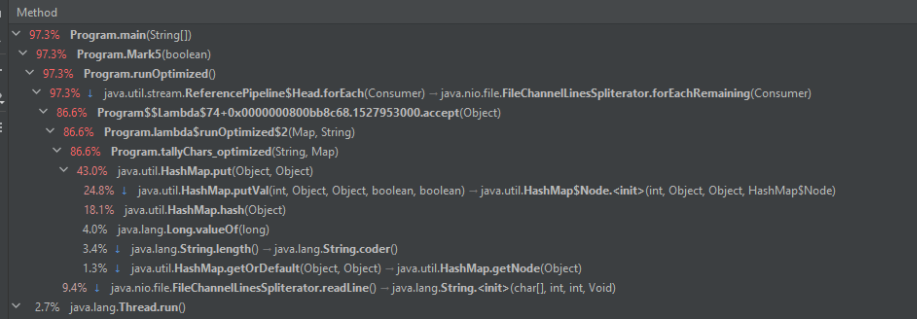
\includegraphics[width = 0.8\textwidth ]{figures/profile4.PNG}
    \caption{Java Fligt Recorder Profile 4}
    \label{fig:p4}
\end{figure}

\subsection{Comparison}
This section goes into detail of the speed improvements.

\begin{figure}[H]
    \centering\
    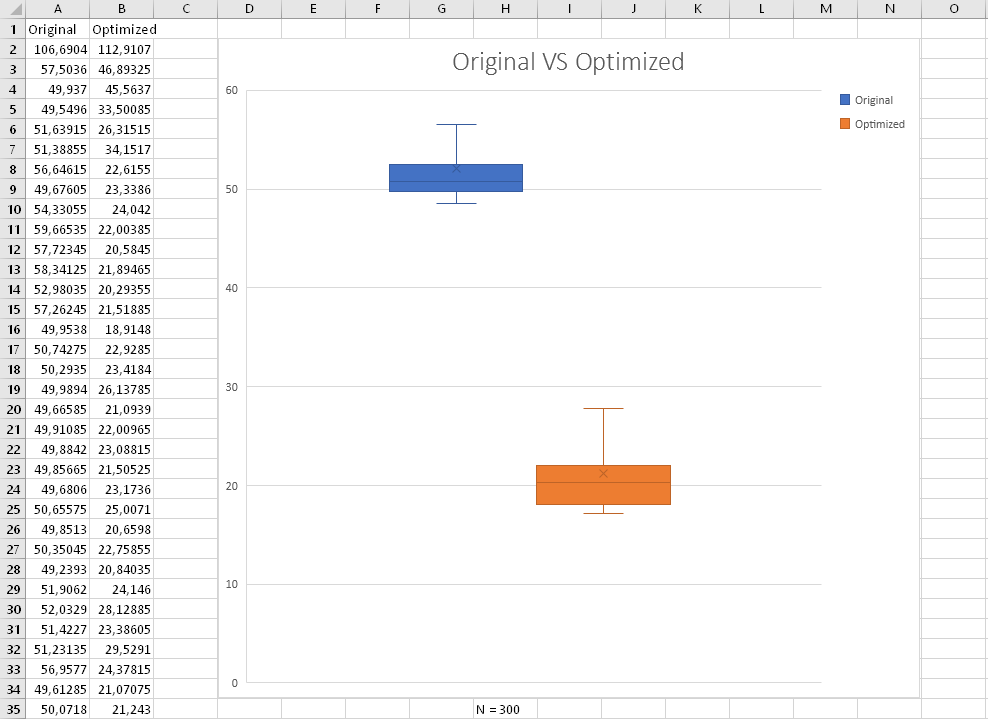
\includegraphics[width = 0.95\textwidth ]{figures/boxplots.png}
    \caption{Boxplot of performance between original and optimized solution}
    \label{fig:boxplots}
\end{figure}



\newpage
\vspace{0.5cm}

